\documentclass[a4paper]{article}
\usepackage[utf8]{inputenc}
\usepackage[english, magyar]{babel}
\usepackage{t1enc}
\usepackage{graphicx} % Required for inserting images

\usepackage[style=ieee]{biblatex}
\usepackage{csquotes}
\addbibresource{hivatkozasok.bib}

\title{Az univerzum múltja, jövője, kulturálisan és tudományosan}
\author{Kékesi Kristóf Mihály (ZI6I4M)}
\date{2023. november}

\begin{document}

\maketitle

\section*{Kulturálisan}
Az emberiségnek mindig is megvoltak az eredettörténetei (sőt, egyes esetekben történetek a világ jelenlegi formájának pusztulásáról is), amik a mi jelenlétünkön kívül általában a környezetünk keletkezésére is reflektálnak. A következő bekezdésekben időrendi sorrendben írok pár teremtéstörténetről, és egy legendáról a világ pusztulásáról, majd kifejtek három tudományos elméletet az univerzumum jelenlegi formájának megszűnéséről.

\subsection*{Egyiptomi teremtésmítosz}
Egyiptomban az ókori lakosok politeista vallásban hittek, több istent is imádtak. A vallásuk által leírt teremtésnek két változatát ismerjük, ezek a memphiszi- és a héliopoliszi teológia. A politeista vallás, és a vallás szájhagyomány útján való terjedése miatt a birodalom más-más részein különböző legendákat meséltek. \cite{egyiptologia}
\par
A memphiszi teológiában a világ alkotását Ptah világteremtő isten (\ref{fig:ptah}. ábra) végezte, gondolataival és elméjével, értelmi tevékenység során. Ezzel ellentétben a héliopoliszi teológia a teremtést Atum istennel (\ref{fig:atum}. ábra) hozza kapcsolatba. Az ebbe a körbe tartozó mítoszokban Atum teremtette meg az istenek első generációjat, akik később sokasodva betöltötték a világ egészét. A héliopoliszi teológiába tartozó mítoszok gyakran kötik össze Atum teremtésének alapját a köpéssel, és Atum onániájával, emiatt a memphiszi teológia a kettő közül a műveltebb felfogású. \cite{egyiptomiteologiak}

\begin{figure}
\centering
\begin{minipage}{.5\textwidth}
  \centering
  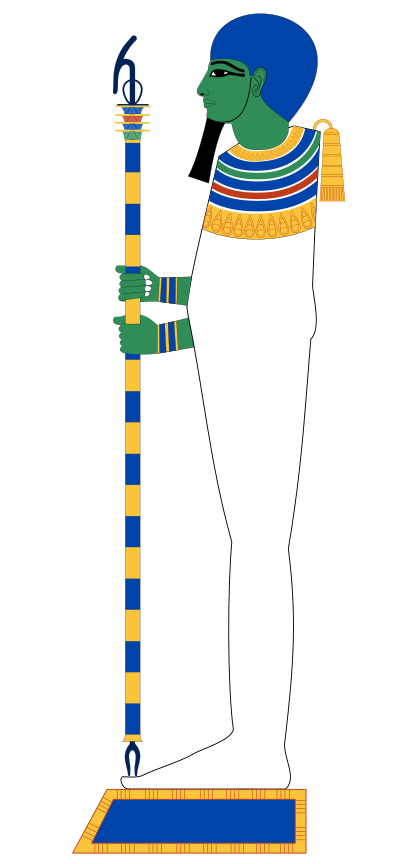
\includegraphics[width=0.4\linewidth]{ptah.png}
  \caption{Ptah ábrázolása}
  \label{fig:ptah}
\end{minipage}%
\begin{minipage}{0.5\textwidth}
  \centering
  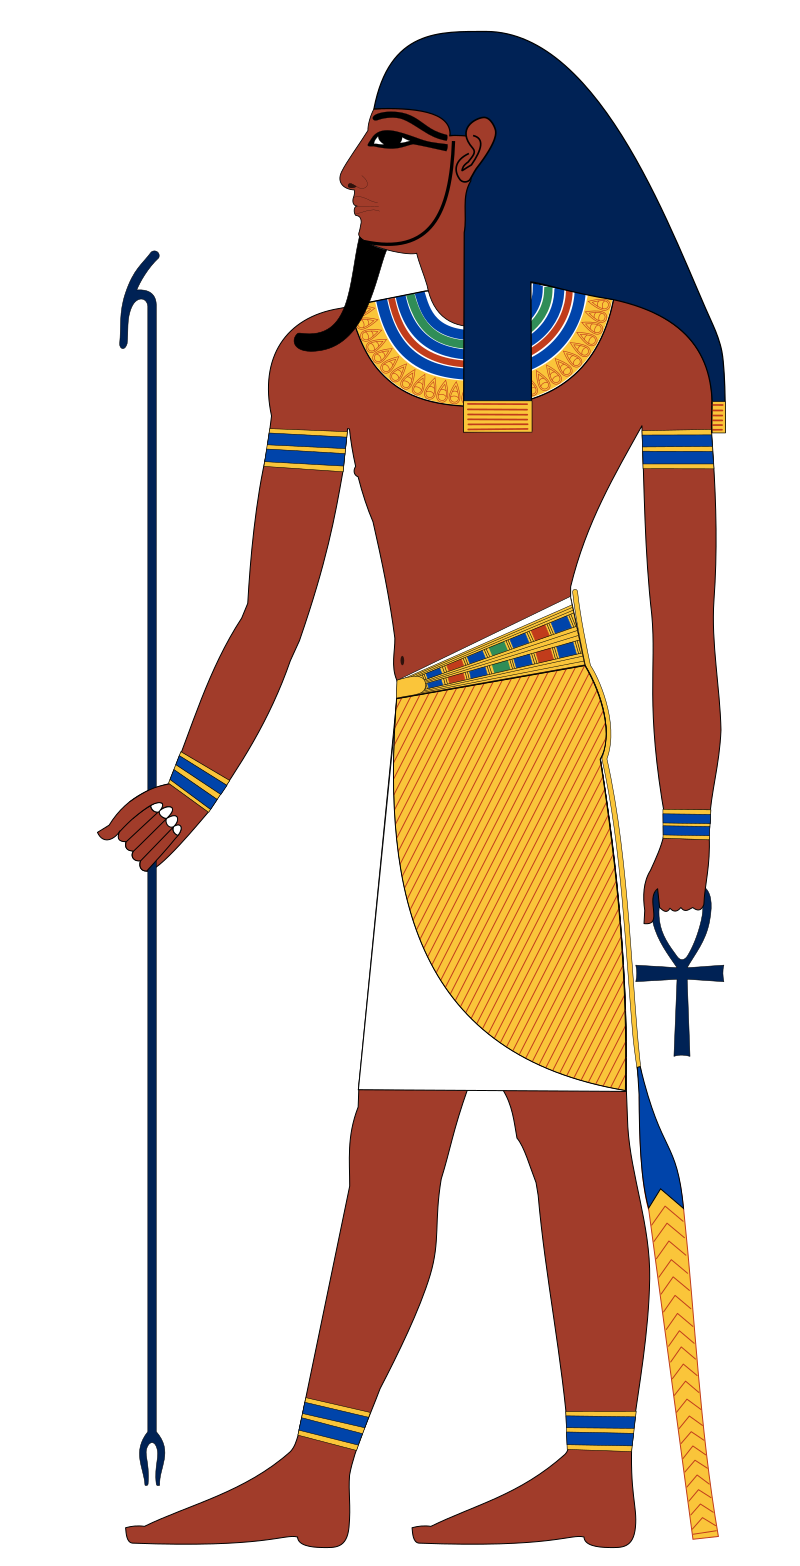
\includegraphics[width=0.4\linewidth]{atum.png}
  \caption{Atum ábrázolása}
  \label{fig:atum}
\end{minipage}
\end{figure}

{
\footnotesize
    Az egyiptomi vallásban a legtöbb istennek megvolt a maga állati formája. Ezalól Ptah kivétel, ami nagy jelentősséggel bír. Ahhoz, hogy megalakuljon a civilizáció, az embereknek kommunikálniuk kell, csoportokba kell letelepedniük, városokat kell építeniük. Ez a folyamat elszakítja az embereket más állatoktól. Ezt jelképezi Ptah kivétele. \cite{egyiptomiteologiak}
}

\subsection*{Bibliai teremtéstörténet}
A Biblia már az első oldalon a teremtéstörténettel kezdődik. Isten hét nap alatt teremtette a földet, ez lehet hat is, attól függ beleszámoljuk-e a hetedik napot, a megpihenést. Amennyiben igen, egy meseszámmal találjuk szembe magunkat, ami a számszimbólika szerint a szentséget jelenti, megszenteli a teremtést.
\par
A teremtés napjait külön-külön nézve az első nap "Kezdetben teremté Isten az eget és a földet." (1Móz 1,1), a sötétséget és a világosságot. Ez felfogható a csillagok teremtésének. A teremtésnek az univerzumra, mint egészre vett része az első nap zajlott le. A teremtés második napján Isten létrehozta az égboltot (értelmezhető az atmoszféraként). Harmadnap megteremtette a szárazföldeket, nevén nevezte a tengerekkel együtt, majd nővényeket teremtett. Negyednap megalkotta a Napot és a Holdat, ötödik nap megalkotta a vízi állatokat a madarakkal együtt, hatodik nap mindenféle egyéb állatokat, majd az embert. "A hetedik napra elkészült Isten a maga alkotó munkájával, és megpihent a hetedik napon az egész alkotó munkája után." (1Móz 2,2). \cite{biblia}
\par
{
    \footnotesize
    A Biblia ködösen fogalmaz a teremtés első napjával kapcsolatban, a földet kisbetűvel írja, így a fent idézett 1Móz 1,1 vehető az űr és a benne lévő anyag teremtésének.
}

\subsection*{Teremtéstörténet a finn mitológiában}
Finnországban a magyar népdalgyűjtéssel egyidőben szintén a nacionalizmus hatására megindult a finn epikus énekek és népi történetek gyűjtése. Ennek következményeképp jött létre a Kalevala, amely tartalmazza a finn mitológiát. Az eposzból kiderül, hogy a teremtés hét tojással kezdődött, melyet egy kacsa rakott Ilmatár, az istennő térdére. (Itt a Bibliához hasonlóan előkerül a hetes szám, ami a számszimbolika szerint szent szám, ez tovább erősíti a teremtés szentségét). Az istennő megtűri a fészket a hét tojással, de mivel a kotlás sok hővel jár levette a lábáról a fészket, ezzel a tojások összetörtek. Ilmatár nem csak pusztító munkát végez, miután kialakultak a tojás különböző részeiből a világunk különböző részei (a föld, az ég, a Hold és a Nap), maga is alkot a tojásokból, megalkotja a különböző földrajzi jellemzőket, a partokat, a szigeteket, zátonyokat és a hegyeket. \cite{kalevala}

\subsection*{Ragnarök, az istenek alkonya}
A skandináv vikingek hittek abban, hogy a világuk ahogyan ismerik véget fog érni egy nap. Ezt nevezték ragnaröknek, az istenek alkonyának. A mítosz szerint a világ végének kezdetét megelőzi egy három éves tél, amely alatt a világon eluralkodnak a háborúk. Maga a ragnarök három kakas kukorékolásával kezdődik a kilenc birodalom három bolygóján. Az esemény alatt minden nép csatába száll egymással, a végső csatára Vígrid mezején kerül sor. Itt majdnem mindenki elpusztul, a háborút csak két ember, egy férfi és egy nő éli túl, Lif és Lifthrasir. Nevük jelentése élet.
\cite{edda, skandinavmitologia}

\section*{Tudományosan}
A jelenlegi számítások alapján a világegyetem 13,8 milliárd évvel ezelőtt jött létre \cite{univerzumkora}, összehasonlítás képpen a Föld 4,45 milliárd éves. \cite{foldkora} Szerencsére a fizika és az elméleti fizika segítségével belátást nyerhetünk hogyan is kezdődött el minden, sőt, még a tudomány jelenlegi álláspontjait követve elméletekkel is megismerkedhetünk, hogy hogyan lesz vége az univerzumunknak.

\subsection*{Ősrobbanás}
A jelenleg elfogadott álláspont az univerzum keletkezéséről az, hogy 13,8 milliárd évvel ezelőtt \cite{univerzumkora} egy végtelenül kicsi és végtelenül forró szingularitásből jött létre minden, egy robbanásszerű esemény hatására. Ezt nevezzük ősrobbanásnak. \cite{big}
\par
{
    \footnotesize
    Az ősrobbanás maradványát, a kozmikus mikrohullámú háttérsugárzást (CMB) még napjainkban is lehet érzékelni. Erre példa amikor a műholdas TVn nincs jel. Az ekkor látott statikus zaj 1\%-át teszi ki a CMB.
}

\begin{figure}
    \centering
    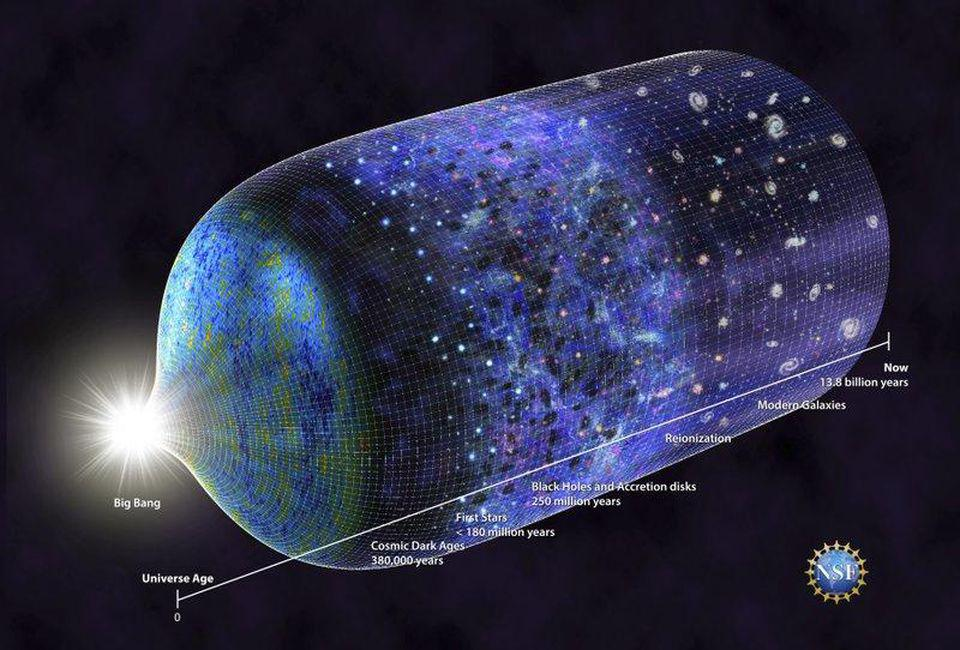
\includegraphics[width=0.75\textwidth]{bigbang.jpg}
    \caption{Az univerzum 13,8 milliárd éve vízualizálva}
    \label{fig:bigbang}
\end{figure}
    
\subsection*{Furcsa anyag}
Közel négy évtizeddel ezelőtt három tudós felvetette, hogy létezhetnek olyan anyagok, amelyeknek a felépítése nem hasonlít a minket körülvevő anyagokéhoz. Ezeket "quark matter"-nek, kvark anyagnak nevezték el. \cite{PhysRevD.30.2379}
\par
A kvark anyagok közül témám szerint kiemelkedik a furcsa anyag. Ez az anyag a számítások szerint neutron csillagok belsejében található.  A szimulációk alapján olyan tulajdonsággal bír, hogyha egy atom hozzáér egy furcsa anyaghoz az is furcsa anyaggá változik. \cite{strange_matter} Ebben rejlik pusztító mivolta, amivel kiérdemelte a helyét az univerzum végéhez vezető események listáján.
\par
{
\footnotesize
A szaknyelvben külön szó van ez elszökött, az űrben sodródó furcsa anyagra, ez a
\begin{otherlanguage}{english}
    "strangelet".
\end{otherlanguage}
}

\subsection*{Hőhalál}
Az univerzumban véges sok anyag és energia található. Feltéve, hogy elég ideig létezik az univerzum, elképzelhető, hogy a világegyetem mindenhol azonos hőmérsékletű, és azonos sűrűségű anyagból fog állni. Amennyiben ez bekövetkezik az univerzum ebben az állapotában fog maradni addig, amíg másmilyen módon vége nem lesz. Ezt nevezzük az univerzum hőhalálának.
\par
Ez hasonló a furcsa anyaghoz, a hőhalál bekövetkezte után se lesz képes az univerzum az élet fenttartásához. A furcsa anyaggal ellentétben a hőhalál beállásával megszűnik minden mozgás a világegyetemben.

\subsection*{Nagy zsugorodás}
Egy másik elmélet szerint az univerzum eléri a maximális kiterjedését, majd a világegyetem tágulása átvált a szűkülésébe addig, amíg egy fordított ősrobbanáshoz hasonlíthatóan minden anyag egy végtelenül kicsi és végtelenül energiadús szingularitásba nem tömörül.

\begin{figure}
    \centering
    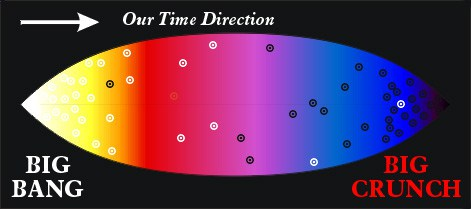
\includegraphics[width=0.75\textwidth]{bigcrunch.jpg}
    \caption{Az univerzum kiterjedésének ábrázolása az ősrobbanástől a nagy zsugorodásáig}
    \label{fig:bigcrunch}
\end{figure}

Az elmélet mögött, hogy miért fog megállni a világegyetem tágulása az áll, hogy az univerzumban lévő összes anyag együttes tömege elég nagy ahhoz, hogy annak a tömegvonzása megállítsa az ősrobbanással elindult növekvést.\cite{big}
\par
{
    \footnotesize
    \Aref{fig:bigcrunch}. ábrán jól megfigyelhető a világegyetem méretének változásával járó vöröseltolódás az univerzum növekedő fázisában, majd a kékeltolódás a szűkülésével. Ennek az oka, hogy ahogyan változik az univerzumunk mérete, úgy változik a benne lévő galaxisok, és galaxishalmazok közötti távolság is. Ennek következményeképp minél messzebbre nézünk az űrben, annál vörösesebbnek hatnak a messzebbről érkező fotonok \cite{redshift}. Ennek oka hasonló a Doppler-effektuséhoz. \cite{doppler}
}

\subsection*{Fentiek kombinálása}
Semmi nem zárja ki, hogy csak egyféleképpen érhet véget az univerzum. Elképzelhető, hogy a fent említettek elméletek mindegyike megtörténjen. Ebben az esetben ezek a katasztrófák csak az alábbi sorrendben történhetnek meg:
\begin{enumerate}
        \item Furcsa anyag
        \item Hőhalál
        \item Nagy zsugorodás.
\end{enumerate}
\par
{
\footnotesize
    Magyarázat: Mivel a nagy zsugorodás egy szingularitásba tömöríti a világegyetemet, ezért ha egymás után következnének be ezek az események, ennek kellene az utolsónak lennie, hogy a többi is bekovetkezhessen. Mivel a hőhalál után semmiféle mozgás nem lehetséges az univerzumban, nem tudna a furcsa anyag terjedni, ezért a furcsa anyagnak kell az első katasztrófának lennie, és a hőhalálnak a másodiknak.
}

\printbibliography
\end{document}
